\documentclass[conference]{IEEEtran}
\usepackage{amsmath, amssymb}
\usepackage{graphicx}
\usepackage{booktabs}
\usepackage{array}
\usepackage{hyperref}
\usepackage{tikz}
\usetikzlibrary{arrows.meta, positioning}

\title{An IEEE Conference Paper Template Written in \LaTeX}

\author{
\IEEEauthorblockN{First Author}
\IEEEauthorblockA{Department of Computer Science\\
Example University\\
first.author@example.edu}
\and
\IEEEauthorblockN{Second Author}
\IEEEauthorblockA{School of Artificial Intelligence\\
Example Institute of Technology\\
second.author@example.edu}
}

\begin{document}
\maketitle

\begin{abstract}
This template follows the IEEE conference two-column format using the
\texttt{IEEEtran} document class. It demonstrates abstract, sections,
equations, figures, tables, and IEEE-style references. Replace the content
with your own research.
\end{abstract}

\begin{IEEEkeywords}
LaTeX, IEEEtran, conference paper, template
\end{IEEEkeywords}

\section{Introduction}
IEEE conferences require a specific two-column layout. This template ships
with \texttt{IEEEtran} and compiles out of the box. Cite prior work
as~\cite{ieee_demo}.

\section{Method}
Consider the objective
\begin{equation}
  \mathcal{L}(\theta) = \frac{1}{N}\sum_{i=1}^{N}
  \ell\!\left(f_\theta(x_i), y_i\right) + \lambda \|\theta\|_2^2,
\end{equation}
where $f_\theta$ is the model and $\ell$ the loss function.

\begin{figure}[htbp]
  \centering
  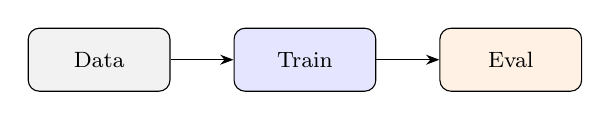
\begin{tikzpicture}[scale=0.9, every node/.style={font=\footnotesize}]
    \node[draw, rounded corners, fill=gray!10, minimum width=1.8cm, minimum height=0.8cm] (a) {Data};
    \node[draw, rounded corners, fill=blue!10, minimum width=1.8cm, minimum height=0.8cm, right=0.8cm of a] (b) {Train};
    \node[draw, rounded corners, fill=orange!10, minimum width=1.8cm, minimum height=0.8cm, right=0.8cm of b] (c) {Eval};
    \draw[-{Stealth}] (a) -- (b);
    \draw[-{Stealth}] (b) -- (c);
  \end{tikzpicture}
  \caption{Workflow of the proposed approach.}
  \label{fig:workflow}
\end{figure}

\section{Experiments}
Table~\ref{tab:comparison} compares illustrative results.

\begin{table}[htbp]
  \centering
  \caption{Comparison with baselines.}
  \label{tab:comparison}
  \begin{tabular}{lcc}
    \toprule
    Model & Top-1 (\%) & Params (M) \\
    \midrule
    ResNet-50 & 76.1 & 25.6 \\
    Ours      & \textbf{79.4} & 24.8 \\
    \bottomrule
  \end{tabular}
\end{table}

\section{Conclusion}
An IEEE-ready starting point for your next submission.

\begin{thebibliography}{1}
\bibitem{ieee_demo}
IEEE Editorial Staff.
\newblock ``IEEE author guidelines,''
\newblock \emph{IEEE Transactions}, vol.~1, no.~1, pp.~1--10, 2024.
\end{thebibliography}

\end{document}
